\section{Deskripsi Penugasan}\label{sec:Pendahuluan} % (fold)
\begin{figure}[htbp]
    \begin{center}
        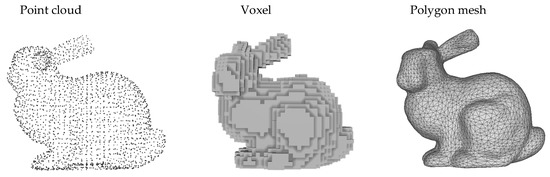
\includegraphics[width=0.5\textwidth]{figures/voxel.jpg}
    \end{center}
    \caption{Visualisasi \textit{Voxelization} \\ Sumber:
    \url{https://www.mdpi.com/1424-8220/22/18/7040}}
\end{figure}

\textit{Voxelization} merupakan proses konversi objek tiga dimensi
yang umum menjadi sebuah model yang tersusun dari kubus-kubus kecil
seperti di Minecraft. Proses konversi ini dilakukan dengan
memanfaatkan struktur data \textbf{Octree}, yaitu sebuah
\textit{tree} yang setiap percabangan terdiri dari 8 anak. Melalui
\textit{Octree}, sebuah ruang kubus 3D dapat dipotong menjadi 8 kubus
berbeda, yang masing-masing dapat dipotong lagi menjadi 8 kubus yang
lebih kecil.

\begin{figure}[htbp]
    \begin{center}
        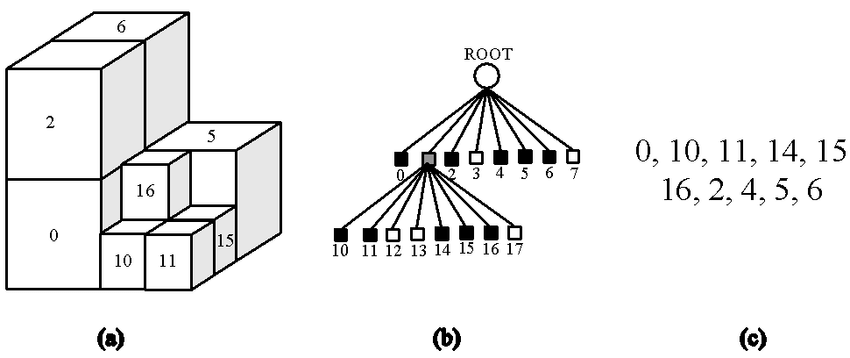
\includegraphics[width=0.5\textwidth]{figures/octree.png}
        \caption{Visualisasi \textit{Octree} terhadap 3D Model}
        Sumber: \\
        \url{https://www.researchgate.net/figure/a-Octants-b-Octree-Structure-c-Linear-Octree-Each-of-the-cubes-has-a-locational-code_fig1_221115507}
    \end{center}
\end{figure}

Tugas Anda adalah mengimplementasikan sebuah program yang dapat
mengkonversi model .obj yang umum menjadi model .obj yang terdiri
dari \textit{voxel} dengan memanfaatkan properti \textit{Octree}.
Program melakukan konversi model dengan menggunakan algoritma
\textbf{\textit{divide and conquer}}.

% section Pendahuluan (end)

\section{Ilustrasi Kasus}\label{sec:Ilustrasi Kasus} % (fold)
Diberikan sebuah model 3D sebagai berikut.
\begin{figure}[htbp]
    \begin{center}
        
\includegraphics[width=0.5\textwidth]{figures/input.png}
    \end{center}
\end{figure}

\noindent Di bawah ini adalah hasil perubahan.
\begin{figure}[htbp]
    \begin{center}
        
\includegraphics[width=0.5\textwidth]{figures/output.png}
    \end{center}
\end{figure}
% section Ilustrasi Kasus (end)

\section{Spesifikasi Tugas}\label{sec:Spesifikasi Tugas} % (fold)
\subsection{Spesifikasi Wajib}\label{sub:Spesifikasi Wajib} % (fold)
\begin{itemize}[leftmargin=*]
    \item Buatlah sebuah program dalam bahasa \textbf{Go, C, C++,
        atau Java} yang mengimplementasikan \textbf{algoritma
        \textit{Divide and Conquer}} untuk melakukan konversi model
        tiga dimensi.
    \item Output voxel harus berukuran \textbf{uniform}, diambil dari
        \textit{leaf} pada \textit{depth} maksimum.
    \item Transformasi hanya perlu dilakukan pada permukaan objek.
    \item Tugas dikerjakan \textbf{berkelompok} dengan anggota
        \textbf{2 orang}, boleh lintas kelas maupun kampus.
    \item \textbf{Input:} Program menerima \textit{path} dari sebuah
        file \texttt{.obj} yang ingin dikonversi dan juga tingkat
        kedalaman pohon maksimum. Untuk tugas besar ini,
        \textbf{hanya memperhatikan nilai x, y, z pada
        \textit{vertice} v, dan \textit{faces} f.} Program harus bisa
        menentukan apakah input valid atau tidak. Format
        \texttt{.obj} valid adalah \textit{row-row} yang berisikan
        \texttt{<v x y z>} atau \texttt{<f i j k>}.

        Contoh konten \texttt{.obj}:
        \begin{tcolorbox}[colback=white, colframe=black, sharp
            corners, boxrule=0.5pt]
\begin{verbatim}
v  2.229345 -0.992723 -0.862826
v  2.292449 -0.871852 -0.882400
v  2.410367 -0.777999 -0.841105
f 1 2 3
    \end{verbatim}
        \end{tcolorbox}

    \item \textbf{Output:} Program mengembalikan:
        \begin{itemize}
            \item sebuah file \texttt{.obj} yang merupakan hasil konversi;
            \item Di CLI, program harus menampilkan setidaknya
                informasi-informasi berikut:
                \begin{itemize}
                    \item Banyaknya voxel yang terbentuk
                    \item Banyaknya vertex yang terbentuk
                    \item Banyaknya faces yang terbentuk
                    \item Statistik \textit{node octree} yang
                        terbentuk dalam format:
                        \begin{tcolorbox}[colback=white,
                            colframe=black, sharp corners, boxrule=0.5pt]
            \begin{verbatim}
1 : <banyaknya node dengan depth 1 yang terbentuk>
2 : <banyaknya node dengan depth 2 yang terbentuk>
...
N : <banyaknya node dengan depth n yang terbentuk>
            \end{verbatim}
                        \end{tcolorbox}
                    \item Statistik node yang \textbf{tidak perlu}
                        ditelusuri dalam format:
                        \begin{tcolorbox}[colback=white,
                            colframe=black, sharp corners, boxrule=0.5pt]

            \begin{verbatim}
1 : <banyaknya node dengan depth 1 yang tidak perlu ditelusuri>
2 : <banyaknya node dengan depth 2 yang tidak perlu ditelusuri>
...
N : <banyaknya node dengan depth n yang tidak perlu ditelusuri>
            \end{verbatim}
                        \end{tcolorbox}
                    \item Kedalaman \textit{octree}
                    \item Lama waktu program berjalan
                    \item \textit{Path} dimana file \texttt{.obj} disimpan
                \end{itemize}
        \end{itemize}
\end{itemize}

% subsection Spesifikasi Wajib (end)

\subsection{Spesifikasi Bonus}\label{sub:Spesifikasi Bonus} % (fold)
Poin maksimal untuk bonus adalah 10. Silahkan pilih spesifikasi bonus
yang akan dikerjakan.
\begin{itemize}[leftmargin=*]
    \item Menggunakan \textit{concurrency} dalam bahasa pemrograman
        yang dipilih untuk algoritma konversi (max 5 poin)
    \item Mengimplementasikan \texttt{.obj} viewer minimal
        menampilkan model 3D hasil \textit{voxelization} secara
        interaktif dalam bahasa pemrograman yang dipilih untuk
        menampilkan hasil objek yang dikonversi (max 10 poin)
\end{itemize}

% subsection Spesifikasi Bonus (end)
% section Spesifikasi Tugas (end)

\section{Dasar Teori}\label{sec:Dasar Teori} % (fold)
\subsection{Algoritma Divide and Conquer}
Algoritma Divide and Conquer merupakan strategi penyelesaian masalah
yang bekerja dengan membagi suatu persoalan besar menjadi beberapa
upa-persoalan yang lebih kecil namun memiliki karakteristik yang
serupa dengan persoalan semula. Proses ini dilakukan secara rekursif
melalui tiga tahapan utama, yaitu Divide untuk membagi masukan,
Conquer untuk menyelesaikan upa-persoalan secara langsung atau
rekursif, serta Combine untuk menggabungkan kembali solusi-solusi
tersebut menjadi satu kesatuan solusi utuh.

\subsection{Voxelization}\label{sub:Voxelization} % (fold)
\textit{Voxelization} merupakan metode transformasi objek tiga
dimensi yang bersifat kontinu, menjadi model tiga dimensi yang
tersusun atas kubus-kubus kecil yang disebut dengan \textit{voxel}.
Proses ini bertujuan agar objek dapat diolah lebih mudah
direpresentasikan di ruang digital.
% subsection Voxelization (end)

\subsection{Octree}\label{sub:Octree} % (fold)
Struktur data Octree merupakan representasi pohon di mana setiap
simpul internal memiliki tepat delapan anak. Masing-masing simpul ini
melambangkan bagian dari sebuah bangun ruang tiga dimensi. Sebuah
kubik dapat dipotong menjadi delapan subkubus yang lebih kecil lagi
sehingga tiap bagian tersebut mencapai tingkat kedalaman yang diinginkan.
% subsection Octree (end)

\subsection{File .obj}\label{sub:File .obj} % (fold)
Format file .obj adalah format representasi yang menyimpan
data model tiga dimensi. Informasi utama yang
disimpan dalam format .obj ini merupakan koordinat verteks (v) yang
menentukan titik-titik dalam model
dan definisi faces (f) yang menyusun permukaan poligon dari verteks
yang tersedia.

Berikut merupakan contoh representasi konten dalam file .obj.

\begin{tcolorbox}[colback=white,
    colframe=black, sharp corners, boxrule=0.5pt]
    \begin{verbatim}
v 2.229345 -0.992723 -0.862826
v 2.292449 -0.871852 -0.882400
v 2.410367 -0.777999 -0.841105
f 1 2 3
    \end{verbatim}
\end{tcolorbox}
% subsection File .obj (end)

\subsection{Concurrency dalam Go}\label{sub:Concurrency dalam Go} % (fold)
Penerapan \textit{concurrency} dalam bahasa pemrograman Go
memungkinkan pengolahan data \textit{Octree} dilakukan secara
paralel, sehingga mengoptimalkan penggunaan sumber daya perangkat
keras pada sistem multi-inti. Berbeda dengan model
\textit{multithreading} pada Java yang menggunakan objek
\textit{Thread} dengan alokasi memori besar, Go menggunakan
\textit{goroutines} yang sangat ringan dan dikelola oleh
\textit{runtime} Go[cite: 3]. Sinkronisasi antar proses dilakukan
menggunakan \texttt{sync.WaitGroup} untuk koordinasi penyelesaian
tugas dan \texttt{sync.Mutex} untuk melindungi integritas data
statistik bersama dari fenomena \textit{race condition}[cite: 3].

\textit{Concurrency} merupakan kemampuan program untuk menangani
berbagai tugas secara bersamaan melalui dekomposisi proses yang
independen. Dalam ekosistem Go, konsep ini diimplementasikan melalui
goroutines. Hal ini memungkinkan sebuah aplikasi menjalankan ribuan
hingga jutaan eksekusi paralel tanpa membebani sistem
secara signifikan.

Berikut adalah potongan implementasi untuk \textit{concurrency} dalam bahasa Go. 

\begin{lstlisting}[language=Java, basicstyle=\ttfamily\small, breaklines=true]
go func() {
    // Sinkronisasi menggunakan WaitGroup
    var wg sync.WaitGroup
    wg.Add(1)
    
    // Pemanggilan fungsi secara concurrent
    go BuildOctreeConcurrent(node, vertices, faces, currentDepth, maxDepth, stats, &wg)
    
    // Menunggu seluruh proses selesai
    wg.Wait()
}
\end{lstlisting}
% subsection Concurrency dalam Go (end)
% section Dasar Teori (end)
